%\chapter{Theoretical background - S}
%	 - Was sind Web-Frameworks
%    - Vor- und Nachteile
%    - Einführung in JavaScript-Frameworks: Allgemeine Informationen zu JavaScriptFrameworks
%    - Kurze Beschreibung Angular.js: Ursprung, Entwicklung, Hauptmerkmale
%    - Kurze Beschreibung Vue.js: Ursprung, Entwicklung, Hauptmerkmale
%    - Was sind die Unterschiede zwischen Angular.js und Vue.js

%\section{What are WebFrameworks} % muss später übersetzt werden

% zitiert aus:
% Ionos. Webfameworks - Überblick und Klassifizierung. Website, Oktober 2022. Online erhältlich unter https://www.ionos.de/digitalguide/websites/web-entwicklung/webframeworks-ein-ueberblick/; abgerufen am 31.05.2024.

% Ein Framework ist ein Programmgerüst, das als Grundlage bei Software-Entwicklungen dient. Frameworks enthalten bereits zahlreiche Funktionen in der Software-Entwicklung als Lösungsvorschläge für individuelle Problemstellungen von verschiedenen Entwicklern. So müssen diese nicht von Null beginnen, wenn sie eie neue Software schreiben möchten.

% Ein Framework beschreibt eine Sammlung an zusammenwirkenden Klassen und fixiert somit auch die Designstruktur für Software, die auf Basis des Frameworks entwickelt wird. 

% Fungiert ein Framework als Grundlage für Web-Anwendungen, spricht man von einem Web-Application-Framework.

%A framework is a program skeleton that serves as a foundation for software development. Frameworks already contain numerous functions in software development as proposed solutions for individual problems faced by various developers. This way, they do not have to start from scratch whenever they want to write new software.

%A framework describes a collection of interacting classes and thus also fixes the design structure for software developed based on the framework.

%If a framework serves as the foundation for web applications, it is referred to as a web application framework.

%\section{WebFrameworks - Pros and Cons}

% zitiert aus:
% Ionos. Webfameworks - Überblick und Klassifizierung. Website, Oktober 2022. Online erhältlich unter https://www.ionos.de/digitalguide/websites/web-entwicklung/webframeworks-ein-ueberblick/; abgerufen am 31.05.2024.

% Webframeworks bieten sehr viele Vorteile, jedoch verbergen auch signifikante Nachteile.

%Web frameworks offer many advantages, but they also hide significant disadvantages.

%\subsection{Advantages}

% zitiert aus:
% Ionos. Webfameworks - Überblick und Klassifizierung. Website, Oktober 2022. Online erhältlich unter https://www.ionos.de/digitalguide/websites/web-entwicklung/webframeworks-ein-ueberblick/; abgerufen am 31.05.2024.

% Die Nutzung von Webframeworks zielt darauf ab, den Zeit- und Kostenaufwand in der Softwareentwicklung zu reduzieren. Der Fokus liegt auf der Wiederverwendung von Code für grundlegende Funktionen wie Datenbankanbindung, Templates, Caching und Sicherheit, die als vorgefertigte Module bereitgestellt werden.

% Dadurch kann sich die Entwicklung auf den spezifischen Code der neuen Anwendung konzentrieren. Da die meisten Webframeworks als Open-Source verfügbar sind, entstehen in der Regel keine Lizenzkosten.

% Frameworks fördern zudem die Erstellung von sauberem und wartbarem Code, da Entwickler auf bewährte Bausteine zurückgreifen können. Diese werden regelmäßig von der Community verbessert und Sicherheitslücken schnell behoben.

%The use of web frameworks aims to reduce time and cost in software development. The focus is on reusing code for basic functions such as database connections, templates, caching and security, which are provided as pre-built modules.

%This allows development to concentrate on the specific code of the new application. Since most web frameworks are available as open-source, there are generally no licensing costs.

%Frameworks also promote the creation of clean and maintainable code, as developers can rely on proven building blocks. These are regularly improved by the community and security vulnerabilities are quickly addressed.

%\subsection{Disadvantages}

% zitiert aus:
% Ionos. Webfameworks - Überblick und Klassifizierung. Website, Oktober 2022. Online erhältlich unter https://www.ionos.de/digitalguide/websites/web-entwicklung/webframeworks-ein-ueberblick/; abgerufen am 31.05.2024.

% Im Internet stehen zahlreiche Frameworks für die Webentwicklung zur Auswahl, die sich in ihren Designprinzipien und ihrem Funktionsumfang unterscheiden. Je nach Projekt kann ein bestimmtes Framework erforderlich sein, was Kompromisse mit sich bringen kann.

% Frameworks sind zwar als allgemeine Lösungen gedacht, aber Entwickler nutzen oft nicht alle verfügbaren Funktionen, was zu unnötigem Code führen kann, der als Ballast bezeichnet wird.

% Ein weiterer Nachteil ist die Abhängigkeit vom Framework und seinem Anbieter, sowie mögliche Lizenzbeschränkungen. Probleme können auch auftreten, wenn die Weiterentwicklung des Frameworks eingestellt wird. Entwickler müssen sich außerdem in die Struktur und Nutzung des Frameworks einarbeiten, was Zeit erfordert, die jedoch durch vorgefertigte Funktionen und Codebausteine kompensiert wird.

% Da der Quellcode vieler Webframeworks öffentlich zugänglich ist, kann jeder ihn einsehen. Dies kann zu Sicherheitsrisiken führen, besonders wenn Unternehmensanwendungen auf öffentlichem Code basieren.

%On the internet, there are numerous frameworks available for web development, which differ in their design principles and functionality. Depending on the project, a specific framework may be required, which can involve compromises.

%Although frameworks are intended as general solutions, developers often do not use all the available functions, leading to unnecessary code, known as bloat.

%Another disadvantage is the dependency on the framework and its provider, as well as potential licensing restrictions. Problems can also arise if the development of the framework is discontinued. Developers must also familiarize themselves with the structure and use of the framework, which requires time, although this is compensated by pre-built functions and code modules.

%Since the source code of many web frameworks is publicly accessible, anyone can view it. This can lead to security risks, especially if enterprise applications are based on public code.

%\section{Introduction to JavaScript Frameworks}

% zitiert aus:
% Ionos. Die beliebtesten JavaScript-Frameworks und -Bibliotheken. Website, März 2023. Online erhältlich unter https://www.ionos.at/digitalguide/websites/web-entwicklung/beliebte-javascript-frameworks-und-bibliotheken/; abgerufen am 31.05.2024.

% JavaScript ist eine einfach gehaltene Programmiersprache, die sich besonders für die Arbeit im Webbrowser eignet. Doch die Schnittstelle zur Website, das DOM (Document Object Model), kann für viele Programmierer eine Herausforderung darstellen. An dieser Stelle kommen JavaScript-Frameworks und -Bibliotheken ins Spiel: Sie bieten Entwicklern Hilfsmittel, um diese und andere Aspekte der Programmierung zu vereinfachen.

% JavaScript Frameworks sind besonders für die Entwicklung komplexer Webanwendungen geeignet. Wenn sich Entwickler mit den Konzepten und Vorgaben des jeweiligen Frameworks vertraut machen, können sie äußerst effektiv damit arbeiten.

%JavaScript is a straightforward programming language particularly suited for working in web browsers. However, the interface to the website, the DOM (Document Object Model), can pose a challenge for many programmers. This is where JavaScript frameworks and libraries come into play: they provide developers with tools to simplify this and other aspects of programming.

%JavaScript frameworks are especially suitable for developing complex web applications. When developers become familiar with the concepts and guidelines of a particular framework, they can work very effectively with it.

%\section{Short description of Angular.js}

% zitiert aus:
% Angular.de. Was sind Angular und AngularJS?. Website, März 2017. Online erhältlich unter https://angular.de/artikel/was-ist-angular/; abgerufen am 31.05.2024.

% AngularJS, von Google entwickelt, ist ein JavaScript-Framework für die Webentwicklung, das Wert auf Struktur und Qualität legt. Es war das erste Framework, das sich mit Architektur, Testbarkeit und isolierten Komponenten auch für große Enterprise-Anwendungen eignete. Durch Techniken wie Dependency Injection ermöglicht es effiziente und wartbare Softwareentwicklung auf JavaScript-Basis.

% Angular ist eine Weiterentwicklung von AngularJS, wobei die Code-Basis komplett neu geschrieben wurde und nun TypeScript als Grundlage dient. Dies ermöglicht eine Migration oder sogar einen hybriden Einsatz der Versionen. Das Projekt hat sich von der Entwicklung eines reinen Frameworks zu einer umfassenden Plattform für Webanwendungen weiterentwickelt.

%AngularJS, developed by Google, is a JavaScript framework for web development that emphasizes structure and quality. It was the first framework suitable for large enterprise applications, addressing architecture, testability and isolated components. Techniques like dependency injection enable efficient and maintainable software development based on JavaScript.

%Angular is an evolution of AngularJS, with a completely rewritten codebase now using TypeScript as its foundation. This allows for migration or even hybrid use of the versions. The project has evolved from the development of a pure framework to a comprehensive platform for web applications.

%\section{Short description of Vue.js}

% zitiert aus:
% vuejs.org. Einführung. Website. Online erhältich unter https://vuejs.org/guide/introduction.html; abgerufen am 31.05.2024.

% Vue.js (ausgesprochen /vju/, wie "view") ist ein JavaScript-Framework zur Gestaltung von Benutzeroberflächen. Es basiert auf Standard-HTML, CSS und JavaScript und bietet ein deklaratives, komponentenbasiertes Programmiermodell, das es ermöglicht, Benutzeroberflächen jeder Komplexität effizient zu entwickeln.

%Vue.js (pronounced /vju/, like "view") is a JavaScript framework for designing user interfaces. It is based on standard HTML, CSS, and JavaScript and offers a declarative, component-based programming model that allows for the efficient development of user interfaces of any complexity.

%\section{What are the differences between Angular.js and Vue.js}

% zitiert aus:
% kinsta.com. Angular vs. Vue: Ein Kopf-an-Kopf-Vergleich. Website, Juli 2023. Online erhältlich unter https://kinsta.com/de/blog/angular-vs-vue/#angular-vs-vue-hnlichkeiten-und-gemeinsamkeiten; abgerufen am 31.05.2024.

% Angular und Vue.js sind beide JavaScript-Frameworks, die zur Entwicklung moderner Webanwendungen verwendet werden können. Ein Hauptunterschied besteht darin, dass Angular eine MVC-Architektur verwendet, während Vue.js ein progressiveres Framework ist. Angular bietet eine robuste und erprobte Entwicklungsumgebung mit Funktionen wie effizienter Zwei-Wege-Datenbindung, einem umfangreichen CLI und einer gut definierten Architektur. Vue.js hingegen ist flexibler und leichtgewichtiger, mit Funktionen wie dem virtuellen DOM, CSS-Übergängen und einfacheren Berechnungen von Eigenschaften. Beide Frameworks haben ihre Vor- und Nachteile, und die Wahl zwischen ihnen hängt von den spezifischen Anforderungen und Präferenzen eines Projekts ab.

%Angular and Vue.js are both JavaScript frameworks that can be used to develop modern web applications. A key difference is that Angular uses an MVC (Model-View-Controller) architecture, while Vue.js is a more progressive framework. Angular offers a robust and well-established development environment with features like efficient two-way data binding, a comprehensive CLI, and a well-defined architecture. Vue.js, on the other hand, is more flexible and lightweight, with features like the virtual DOM, CSS transitions and simpler computed properties. Both frameworks have their advantages and disadvantages, and the choice between them depends on the specific requirements and preferences of a project.

% MVC: Model View Controller (eine Softwarearchitektur)
% CLI: Command Line Interface (eine textbasierte Benutzerschnittstelle)
% DOM: Document Object Model (eine Programmierschnittstelle für strukturierte Dokumente wie HTML und XML)
% CSS: Cascading Style Sheets (eine Stylesheet-Sprache für die Gestaltung von Dokumenten)

\chapter{Theoretical Background - S}

\section{Web Frameworks}

A framework is a program skeleton that serves as a foundation for software development. Frameworks already contain numerous functions in software development as proposed solutions for individual problems faced by various developers. This way, they do not have to start from scratch whenever they want to write new software.

A framework describes a collection of interacting classes and thus also fixes the design structure for software developed based on the framework. When a framework serves as the foundation for web applications, it is referred to as a web application framework~\cite{ionos_webframeworks}.

\subsection{Pros and Cons of Web Frameworks}

Web frameworks offer many advantages, but they also come with significant disadvantages.

\textbf{Advantages:}
\begin{itemize}
    \item \textbf{Reduced Development Time and Cost:} By reusing code for basic functions such as database connections, templates, caching, and security, development time is significantly reduced.
    \item \textbf{Open Source:} Most web frameworks are available as open-source, eliminating licensing costs.
    \item \textbf{Clean and Maintainable Code:} Frameworks promote the creation of clean and maintainable code, as developers can rely on proven building blocks.
    \item \textbf{Community Support:} Regular improvements and quick fixes for security vulnerabilities are provided by the community~\cite{ionos_webframeworks}.
\end{itemize}

\textbf{Disadvantages:}
\begin{itemize}
    \item \textbf{Framework-Specific Requirements:} Different frameworks have different design principles, potentially requiring compromises based on the project.
    \item \textbf{Code Bloat:} Developers may not use all available functions, leading to unnecessary code.
    \item \textbf{Dependency Risks:} Reliance on a framework and its provider can be risky if the framework is discontinued or its development slows.
    \item \textbf{Learning Curve:} Familiarizing oneself with a framework’s structure and use takes time.
    \item \textbf{Security Risks:} Publicly accessible source code can pose security risks for enterprise applications~\cite{ionos_webframeworks}.
\end{itemize}

\section{Introduction to JavaScript Frameworks}

JavaScript is a versatile programming language particularly suited for work in web browsers. Originally developed by Netscape, it has become one of the most widely used programming languages on the web, enabling developers to create dynamic and interactive content by manipulating the Document Object Model (DOM).

Direct manipulation of the DOM can be challenging, which is where JavaScript frameworks and libraries come into play. They provide tools to simplify these and other aspects of programming, making JavaScript frameworks especially suitable for developing complex web applications. These frameworks offer a structured approach and pre-built components, enabling more efficient development once the concepts and guidelines of a particular framework are mastered~\cite{ionos_jsframeworks}.

\section{DOM and Dynamic Web Content}

The Document Object Model (DOM) is a programming interface for web documents. It represents the page so that programs can change the document structure, style, and content. The DOM is crucial for creating dynamic web content, which is essential for modern web applications that need to be interactive and responsive~\cite{mdn_dom}.

\subsection{Benefits of Dynamic Web Content}

\begin{enumerate}
    \item \textbf{Personalization}: Tailoring content based on user preferences, demographics, or behavior can significantly boost engagement and conversion rates. Personalized experiences are crucial for retaining visitors and improving user satisfaction.
    
    \item \textbf{Real-time Updates}: Providing timely information without refreshing the entire page is crucial for news websites, social media platforms, and e-commerce sites. JavaScript enables real-time updates through asynchronous requests and data manipulation.
    
    \item \textbf{Enhanced User Engagement}: Interactive features such as live chat, dynamic forms, and multimedia sliders captivate users, extending session duration and reducing bounce rates.
\end{enumerate}

\subsection{Implementing Dynamic Web Content}

To effectively implement dynamic web content using JavaScript and jQuery:

\begin{enumerate}
    \item \textbf{Define Goals}: Clearly outline objectives, whether to enhance user experience, increase conversions, or improve engagement metrics.
    
    \item \textbf{Utilize User Data}: Analyze user behavior with tools like Google Analytics to personalize content and tailor dynamic elements based on preferences and interactions.
    
    \item \textbf{Choose Technologies}: Select appropriate JavaScript frameworks or libraries (e.g., React, Vue.js) and jQuery plugins to streamline development and ensure cross-browser compatibility.
    
    \item \textbf{Test and Iterate}: Continuously test dynamic features, gather user feedback, and refine implementations to optimize performance and user satisfaction.
\end{enumerate}

By leveraging JavaScript and jQuery for dynamic web content, websites can offer personalized, engaging experiences that cater to modern user expectations~\cite{moldstud2024}.

\section {Comparison criteria - M}

When evaluating web development frameworks, metrics play a crucial role as they enable an objective analysis of performance and efficiency. By comparing load times, responsiveness, and resource utilization, frameworks like Angular and Vue can be assessed in various scenarios to determine their performance.

\subsection{Performance}
Angular provides robust performance and scalability for complex applications. In contrast, Vue stands out for its fast loading times and low overhead, making it particularly attractive for smaller projects~\cite{verma2022comparison}.

\subsection{Developer-Friendliness}
Angular offers a robust structure and comprehensive features, which come with a steeper learning curve but are supported by extensive documentation and a strong community. Vue, on the other hand, is characterized by its easy integration and intuitive syntax, facilitating quicker onboarding and flexibility for smaller projects~\cite{angular, vue}.

\subsection{Community Support}
Active and engaged community support is crucial for framework development and bug fixing. Referring to the study by Jelica Cincović and Marija Punt titled "Comparison: Angular vs. React vs. Vue," which examined community support through GitHub repository comparisons, Figure  illustrates the following:

\begin{figure}[h]
    \centering
    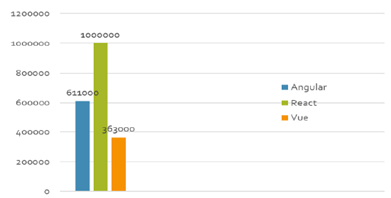
\includegraphics[width=0.6\textwidth]{image.png}
    \caption{Number of GitHub repositories by frameworks}
    \label{fig:github_repos}
\end{figure}

The graph indicates that React enjoys the largest community support, followed by Angular in second place and Vue in third~\cite{cincovic2020comparison}.

\section{JavaScript for Complex Web Applications}

JavaScript is well-suited for complex web applications due to its versatility and the powerful features of modern JavaScript frameworks. These frameworks provide a structured environment for development, making it easier to manage large codebases and maintain code quality.

\textbf{Alternatives to JavaScript:}
\begin{itemize}
    \item \textbf{TypeScript:} A superset of JavaScript that adds static types, making it easier to catch errors early.
    \item \textbf{Dart:} Developed by Google, Dart is used in conjunction with the Flutter framework for building web and mobile apps.
    \item \textbf{Elm:} A functional language that compiles to JavaScript, focused on simplicity and quality tooling~\cite{mdn-js-guide}.
\end{itemize}

\section{Relevant JavaScript Frameworks}

Several JavaScript frameworks are popular for developing web applications, each with its unique features and strengths. This section provides a brief overview of two of the most relevant frameworks, Vue.js and Angular, and explains why they are examined in detail.

%\section{Brief Description of Angular.js}

%AngularJS, developed by Google, is a JavaScript framework for web development that emphasizes structure and quality. It was introduced in 2010 and was the first framework suitable for large enterprise applications, emphasizing clear architecture, high testability, and isolated components. Techniques like Dependency Injection enable efficient and maintainable software development based on JavaScript.

%Angular, introduced in 2016 as a successor to AngularJS, is a complete rewrite and uses TypeScript as its foundation. This allows for better scalability and performance. Angular offers an extensive development environment with features such as two-way data binding, a powerful Command Line Interface (CLI), and a well-defined architecture. It has evolved from a pure framework to a comprehensive platform for developing web applications \cite{angular}.

%\section{Brief Description of Vue.js}

%Vue.js, pronounced /vju:/, like "view", is a JavaScript framework for designing user interfaces. It was developed by Evan You in 2014 and has quickly become one of the most popular frameworks. Vue.js is based on standard HTML, CSS, and JavaScript and offers a declarative, component-based programming model. This model allows for efficient development of user interfaces of any complexity. Key features of Vue.js include the virtual DOM, reactive data binding, and easy integration with other projects and libraries.

%Vue.js is flexible and lightweight, suitable for both small projects and large applications. It allows developers to incrementally adopt it into existing projects and add additional features as needed \cite{vuejs}.

\subsection{Angular}

Angular is a platform and framework for building single-page client applications using HTML and TypeScript. Developed by Google, Angular provides a comprehensive solution for complex and large-scale applications~\cite{angular-io}.

\textbf{Key Features:}
\begin{itemize}
    \item Two-way data binding
    \item Dependency Injection
    \item Comprehensive CLI
    \item TypeScript support
\end{itemize}

\subsection{Vue.js}

Vue.js is a progressive JavaScript framework for building user interfaces. It is designed to be incrementally adoptable and can function as a library or a full-fledged framework. Vue.js is known for its simplicity and flexibility, making it suitable for both small projects and large applications~\cite{vuejs2024}.

\textbf{Key Features:}
\begin{itemize}
    \item Virtual DOM
    \item Reactive data binding
    \item Component-based architecture
    \item Easy integration with other projects and libraries
\end{itemize}

%\section{Differences Between Angular.js and Vue.js}

%Angular and Vue.js are both JavaScript frameworks that can be used to develop modern web applications. A key difference is that Angular uses an MVC (Model-View-Controller) architecture, while Vue.js is a more progressive framework.

%Angular provides a robust and well-established development environment with features such as efficient two-way data binding, a comprehensive CLI, and a well-defined architecture. It is particularly suitable for large and complex applications due to its strict structure and extensive tools.

%On the other hand, Vue.js is more flexible and lightweight. It uses a virtual DOM, which improves performance, and offers simple ways for CSS transitions and property computation. Vue.js is easier to learn and integrate, making it a good choice for smaller projects or projects that require rapid development.

%Both frameworks have their advantages and disadvantages, and the choice between them depends on the specific requirements and preferences of a project. While Angular offers a comprehensive solution for complex applications, Vue.js excels in simplicity and flexibility \cite{kinsta}.

\section{Vue.js vs. Angular: A Detailed Comparison}

In this section, we will compare Vue.js and Angular based on several parameters to provide a clear understanding of their respective strengths and weaknesses.

\subsection{Performance}

\textbf{Vue.js:}
\begin{itemize}
    \item Uses a virtual DOM for efficient updates
    \item Generally faster in rendering due to its lightweight nature
\end{itemize}

\textbf{Angular:}
\begin{itemize}
    \item Real DOM, which can be slower in certain scenarios
    \item Optimized for performance with techniques like ahead-of-time (AOT) compilation
\end{itemize}

\textbf{Comparison:}
\begin{itemize}
    \item Vue.js often has better performance for simple to moderately complex applications.
    \item Angular provides robust performance optimizations suitable for enterprise-level applications.
\end{itemize}

\subsection{Developer-Friendliness}

\textbf{Vue.js:}
\begin{itemize}
    \item Easy to learn and integrate
    \item Simple syntax and flexible structure
    \item Comprehensive documentation
\end{itemize}

\textbf{Angular:}
\begin{itemize}
    \item Steeper learning curve due to its complexity
    \item Requires understanding of TypeScript
    \item Extensive documentation and resources
\end{itemize}

\textbf{Comparison:}
\begin{itemize}
    \item Vue.js is generally more accessible for beginners.
    \item Angular is more suitable for developers with experience in TypeScript and complex frameworks.
\end{itemize}

\subsection{Community Support}

\textbf{Vue.js:}
\begin{itemize}
    \item Growing community with increasing adoption
    \item Numerous plugins and integrations
    \item Active development and support
\end{itemize}

\textbf{Angular:}
\begin{itemize}
    \item Large and established community
    \item Extensive resources and third-party libraries
    \item Backed by Google, ensuring long-term support
\end{itemize}

\textbf{Comparison:}
\begin{itemize}
    \item Angular has a larger and more established community.
    \item Vue.js is rapidly growing and has a supportive community.
\end{itemize}

\subsection{Ecosystem}

\textbf{Vue.js:}
\begin{itemize}
    \item Flexible and integrates well with other libraries
    \item Vue CLI for project scaffolding
    \item Vue Router and Vuex for state management
\end{itemize}

\textbf{Angular:}
\begin{itemize}
    \item Comprehensive suite of built-in tools
    \item Angular CLI for efficient development
    \item Angular Material for UI components
\end{itemize}

\textbf{Comparison:}
\begin{itemize}
    \item Vue.js offers flexibility in choosing tools and libraries.
    \item Angular provides a more integrated and consistent development experience.
\end{itemize}

\section{Conclusion}

Both Vue.js and Angular have their advantages and disadvantages, making them suitable for different types of projects. Vue.js excels in simplicity, flexibility, and ease of integration, making it a good choice for smaller projects or projects that require rapid development. Angular, on the other hand, provides a comprehensive solution for complex and large-scale applications, with a robust set of tools and a well-defined architecture.

The choice between Vue.js and Angular depends on the specific requirements and preferences of a project. Developers should consider factors such as performance needs, developer-friendliness, community support, and the overall ecosystem when making a decision~\cite{kinsta}.